\documentclass[tikz,border=6pt]{standalone}
\usepackage{xcolor}
\usetikzlibrary{arrows.meta,positioning,calc}

% Reproducible paper-style source for assets/diagrams/imu-basketball.svg
% Build from this directory:
%   pdflatex -interaction=nonstopmode -halt-on-error imu-basketball.tex
%   pdftocairo -svg imu-basketball.pdf ../imu-basketball.svg

\definecolor{ink}{HTML}{203746}
\definecolor{muted}{HTML}{657A88}
\definecolor{line}{HTML}{AFC2CE}
\definecolor{panel}{HTML}{F8FAFB}
\definecolor{blue1}{HTML}{E8F1F6}
\definecolor{blue2}{HTML}{C9DDE8}
\definecolor{blue4}{HTML}{4D86A4}
\definecolor{orange}{HTML}{D77A3B}
\definecolor{orangefill}{HTML}{F7E8DE}
\definecolor{green}{HTML}{3E7C73}
\definecolor{greenfill}{HTML}{E4F0ED}

\tikzset{
  >={Stealth[length=2.2mm,width=1.55mm]},
  flow/.style={->,draw=muted,line width=0.85pt},
  radio/.style={->,draw=orange,line width=0.9pt,dashed},
  panelbox/.style={draw=line,fill=panel,rounded corners=2mm,line width=0.65pt},
  panellabel/.style={font=\sffamily\bfseries\small,text=ink},
  body/.style={font=\sffamily\small,text=ink},
  smallbody/.style={font=\sffamily\scriptsize,text=ink},
  sublabel/.style={font=\sffamily\scriptsize,text=muted},
  chip/.style={draw=line,fill=white,rounded corners=1mm,line width=0.6pt,font=\sffamily\scriptsize,text=ink,minimum height=0.62cm},
}

\begin{document}
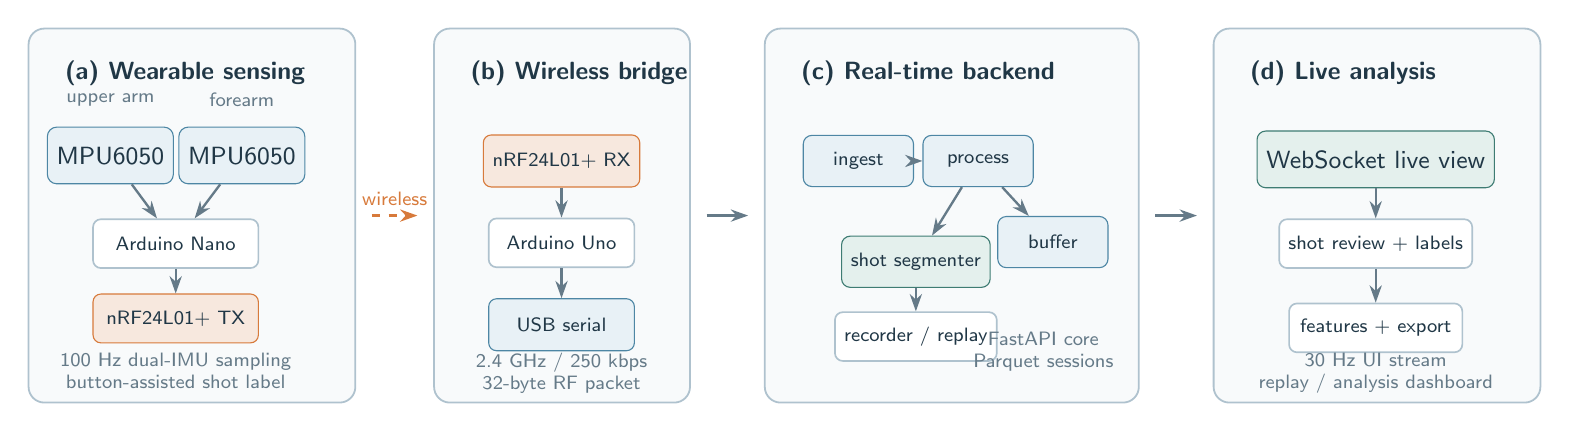
\begin{tikzpicture}[x=1cm,y=1cm]

% (a) Wearable sensing --------------------------------------------------------
\node[panelbox,minimum width=4.15cm,minimum height=4.75cm,anchor=south west] (wear) at (0,0) {};
\node[panellabel,anchor=north west] at ([xshift=3.5mm,yshift=-3mm]wear.north west) {(a) Wearable sensing};

\node[draw=blue4,fill=blue1,rounded corners=1.2mm,minimum width=1.35cm,minimum height=0.72cm,body] (imu1) at (1.05,3.15) {MPU6050};
\node[draw=blue4,fill=blue1,rounded corners=1.2mm,minimum width=1.35cm,minimum height=0.72cm,body] (imu2) at (2.72,3.15) {MPU6050};
\node[sublabel,above=1.3mm of imu1] {upper arm};
\node[sublabel,above=1.3mm of imu2] {forearm};
\node[chip,minimum width=2.10cm] (nano) at (1.88,2.03) {Arduino Nano};
\node[draw=orange,fill=orangefill,rounded corners=1mm,minimum width=2.10cm,minimum height=0.62cm,smallbody] (tx) at (1.88,1.08) {nRF24L01+ TX};
\draw[flow] (imu1) -- (nano);
\draw[flow] (imu2) -- (nano);
\draw[flow] (nano) -- (tx);
\node[sublabel,align=center] at (1.88,0.42) {100 Hz dual-IMU sampling\\button-assisted shot label};

% (b) Wireless bridge ---------------------------------------------------------
\node[panelbox,minimum width=3.25cm,minimum height=4.75cm,anchor=south west] (bridge) at (5.15,0) {};
\node[panellabel,anchor=north west] at ([xshift=3.5mm,yshift=-3mm]bridge.north west) {(b) Wireless bridge};

\node[draw=orange,fill=orangefill,rounded corners=1mm,minimum width=1.85cm,minimum height=0.66cm,smallbody] (rx) at (6.78,3.08) {nRF24L01+ RX};
\node[chip,minimum width=1.85cm] (uno) at (6.78,2.04) {Arduino Uno};
\node[draw=blue4,fill=blue1,rounded corners=1mm,minimum width=1.85cm,minimum height=0.66cm,smallbody] (serial) at (6.78,1.00) {USB serial};
\draw[flow] (rx) -- (uno);
\draw[flow] (uno) -- (serial);
\node[sublabel,align=center] at (6.78,0.39) {2.4 GHz / 250 kbps\\32-byte RF packet};
\draw[radio] ([xshift=2mm]wear.east) -- node[above,sublabel,text=orange] {wireless} ([xshift=-2mm]bridge.west);

% (c) Real-time backend --------------------------------------------------------
\node[panelbox,minimum width=4.75cm,minimum height=4.75cm,anchor=south west] (backend) at (9.35,0) {};
\node[panellabel,anchor=north west] at ([xshift=3.5mm,yshift=-3mm]backend.north west) {(c) Real-time backend};

\node[draw=blue4,fill=blue1,rounded corners=1.1mm,minimum width=1.40cm,minimum height=0.65cm,smallbody] (ingest) at (10.55,3.08) {ingest};
\node[draw=blue4,fill=blue1,rounded corners=1.1mm,minimum width=1.40cm,minimum height=0.65cm,smallbody] (proc) at (12.07,3.08) {process};
\node[draw=blue4,fill=blue1,rounded corners=1.1mm,minimum width=1.40cm,minimum height=0.65cm,smallbody] (buf) at (13.02,2.05) {buffer};
\node[draw=green,fill=greenfill,rounded corners=1.1mm,minimum width=1.72cm,minimum height=0.65cm,smallbody] (seg) at (11.28,1.80) {shot segmenter};
\node[chip,minimum width=1.72cm] (rec) at (11.28,0.85) {recorder / replay};
\draw[flow] (ingest) -- (proc);
\draw[flow] (proc) -- (buf);
\draw[flow] (proc) -- (seg);
\draw[flow] (seg) -- (rec);
\node[sublabel,align=center] at (12.90,0.66) {FastAPI core\\Parquet sessions};
\draw[flow] ([xshift=2mm]bridge.east) -- ([xshift=-2mm]backend.west);

% (d) Live analysis ------------------------------------------------------------
\node[panelbox,minimum width=4.15cm,minimum height=4.75cm,anchor=south west] (ui) at (15.05,0) {};
\node[panellabel,anchor=north west] at ([xshift=3.5mm,yshift=-3mm]ui.north west) {(d) Live analysis};

\node[draw=green,fill=greenfill,rounded corners=1.1mm,minimum width=2.20cm,minimum height=0.72cm,body] (ws) at (17.12,3.10) {WebSocket live view};
\node[chip,minimum width=2.20cm] (shots) at (17.12,2.03) {shot review + labels};
\node[chip,minimum width=2.20cm] (feat) at (17.12,0.96) {features + export};
\draw[flow] (ws) -- (shots);
\draw[flow] (shots) -- (feat);
\node[sublabel,align=center] at (17.12,0.38) {30 Hz UI stream\\replay / analysis dashboard};
\draw[flow] ([xshift=2mm]backend.east) -- ([xshift=-2mm]ui.west);

\end{tikzpicture}
\end{document}
